\documentclass[11pt]{article}
\usepackage[a4paper,margin=22mm]{geometry}
\usepackage[T1]{fontenc}
\usepackage{lmodern}
\usepackage{microtype}
\usepackage{xcolor}
\usepackage{tikz}
\usepackage{hyperref}

\definecolor{graphblue}{HTML}{214F7B}
\definecolor{graphrust}{HTML}{C65D32}
\definecolor{graphgray}{HTML}{707A84}

\tikzset{
  vertex/.style={circle,fill=graphblue,inner sep=2.4pt},
  small vertex/.style={circle,fill=graphblue,inner sep=1.9pt},
  edge/.style={draw=graphblue,line width=0.9pt},
  added edge/.style={draw=graphrust,line width=1.15pt},
  guide/.style={draw=graphgray!55,dashed,line width=0.7pt},
  terminal/.style={circle,draw=graphblue,fill=white,line width=0.9pt,
    minimum size=6mm,font=\small}
}

\newcommand{\classheading}[1]{%
  \par\medskip
  {\large\bfseries #1}\par
  \smallskip
}
\newcommand{\classnote}[1]{%
  \begin{center}
  \begin{minipage}{0.78\linewidth}
  \small #1
  \end{minipage}
  \end{center}
  \medskip
}

\title{Planar Graph Classes: Visual Guide}
\author{Clemens Kuske}
\date{}

\begin{document}
\maketitle

\noindent
Each picture is a small representative or construction diagram. It is meant
to clarify the defining shape; it does not replace the formal Lean definition.

% lax begin Lax68.Planar
\classheading{Planar graphs}
\begin{center}
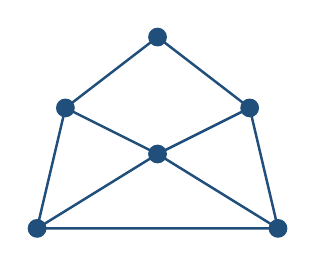
\begin{tikzpicture}[scale=0.9]
  \coordinate (a) at (-1.7,-0.9);
  \coordinate (b) at (1.7,-0.9);
  \coordinate (c) at (1.3,0.8);
  \coordinate (d) at (0,1.8);
  \coordinate (e) at (-1.3,0.8);
  \coordinate (f) at (0,0.15);
  \draw[edge] (a)--(b)--(c)--(d)--(e)--cycle;
  \draw[edge] (a)--(f)--(c);
  \draw[edge] (e)--(f)--(b);
  \foreach \p in {a,b,c,d,e,f} \node[vertex] at (\p) {};
\end{tikzpicture}
\end{center}
\classnote{A planar graph admits a drawing with no two edges crossing away
from their common endpoints.}
% lax end Lax68.Planar

% lax begin Lax68.Outerplanar
\classheading{Outerplanar graphs}
\begin{center}
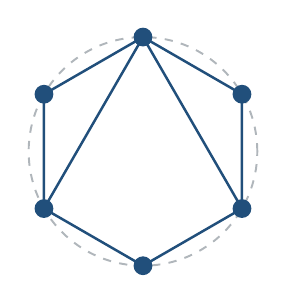
\begin{tikzpicture}[scale=0.88]
  \draw[guide] (0,0) circle (1.65);
  \foreach \i in {0,...,5}
    \coordinate (v\i) at ({90-60*\i}:1.65);
  \draw[edge] (v0)--(v1)--(v2)--(v3)--(v4)--(v5)--cycle;
  \draw[edge] (v0)--(v2) (v0)--(v4);
  \foreach \i in {0,...,5} \node[vertex] at (v\i) {};
\end{tikzpicture}
\end{center}
\classnote{Every vertex lies on the boundary of the outer face; the dashed
circle emphasizes the common boundary.}
% lax end Lax68.Outerplanar

% lax begin Lax68.MaximalOuterplanar
\classheading{Maximal outerplanar graphs}
\begin{center}
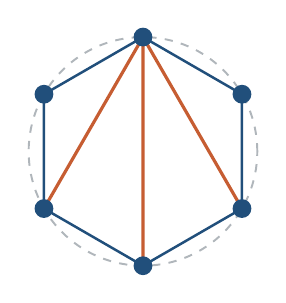
\begin{tikzpicture}[scale=0.88]
  \draw[guide] (0,0) circle (1.65);
  \foreach \i in {0,...,5}
    \coordinate (v\i) at ({90-60*\i}:1.65);
  \draw[edge] (v0)--(v1)--(v2)--(v3)--(v4)--(v5)--cycle;
  \draw[added edge] (v0)--(v2) (v0)--(v3) (v0)--(v4);
  \foreach \i in {0,...,5} \node[vertex] at (v\i) {};
\end{tikzpicture}
\end{center}
\classnote{The boundary polygon is fully triangulated by noncrossing
diagonals. Adding any further edge destroys outerplanarity.}
% lax end Lax68.MaximalOuterplanar

\newpage

% lax begin Lax68.GridsAndWalls
\classheading{Grids and walls}
\begin{center}
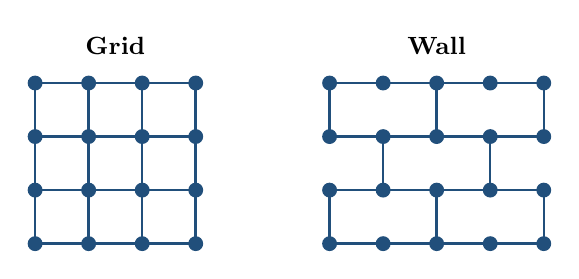
\begin{tikzpicture}[scale=0.68]
  \begin{scope}[xshift=-4.3cm]
    \node[font=\small\bfseries] at (1.5,3.7) {Grid};
    \foreach \x in {0,...,3}
      \foreach \y in {0,...,3}
        \node[small vertex] at (\x,\y) {};
    \foreach \x in {0,...,2}
      \foreach \y in {0,...,3}
        \draw[edge] (\x,\y)--({\x+1},\y);
    \foreach \x in {0,...,3}
      \foreach \y in {0,...,2}
        \draw[edge] (\x,\y)--(\x,{\y+1});
  \end{scope}
  \begin{scope}[xshift=1.2cm]
    \node[font=\small\bfseries] at (2,3.7) {Wall};
    \foreach \x in {0,...,4}
      \foreach \y in {0,...,3}
        \node[small vertex] at (\x,\y) {};
    \foreach \x in {0,...,3}
      \foreach \y in {0,...,3}
        \draw[edge] (\x,\y)--({\x+1},\y);
    \foreach \x in {0,2,4}
      \draw[edge] (\x,0)--(\x,1) (\x,2)--(\x,3);
    \foreach \x in {1,3}
      \draw[edge] (\x,1)--(\x,2);
  \end{scope}
\end{tikzpicture}
\end{center}
\classnote{A grid keeps every horizontal and vertical neighbor edge. A wall
keeps alternating vertical edges, producing the brick pattern.}
% lax end Lax68.GridsAndWalls

% lax begin Lax68.Triangles
\classheading{Triangles}
\begin{center}
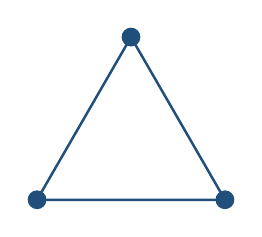
\begin{tikzpicture}[scale=0.95]
  \coordinate (a) at (90:1.45);
  \coordinate (b) at (210:1.45);
  \coordinate (c) at (330:1.45);
  \draw[edge] (a)--(b)--(c)--cycle;
  \foreach \p in {a,b,c} \node[vertex] at (\p) {};
\end{tikzpicture}
\end{center}
\classnote{A triangle is the complete graph on three vertices: every pair of
vertices is adjacent.}
% lax end Lax68.Triangles

% lax begin Lax68.Stars
\classheading{Stars}
\begin{center}

\begin{tikzpicture}[scale=0.88]
  \coordinate (c) at (0,0);
  \foreach \i in {0,...,6} {
    \coordinate (v\i) at ({90-360*\i/7}:1.65);
    \draw[edge] (c)--(v\i);
  }
  \node[vertex] at (c) {};
  \foreach \i in {0,...,6} \node[vertex] at (v\i) {};
\end{tikzpicture}
\end{center}
\classnote{One center is adjacent to every leaf, while no two leaves are
adjacent.}
% lax end Lax68.Stars

% lax begin Lax68.Ladders
\classheading{Ladders}
\begin{center}
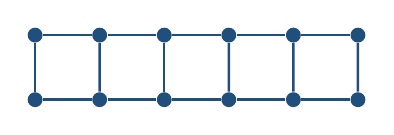
\begin{tikzpicture}[scale=0.82]
  \foreach \x in {0,...,5} {
    \node[small vertex] (t\x) at (\x,1) {};
    \node[small vertex] (b\x) at (\x,0) {};
    \draw[edge] (t\x)--(b\x);
  }
  \foreach \x [evaluate=\x as \y using int(\x+1)] in {0,...,4} {
    \draw[edge] (t\x)--(t\y);
    \draw[edge] (b\x)--(b\y);
  }
\end{tikzpicture}
\end{center}
\classnote{Two paths form the rails, and corresponding vertices are joined
by rungs.}
% lax end Lax68.Ladders

% lax begin Lax68.HalinGraphs
\classheading{Halin graphs}
\begin{center}
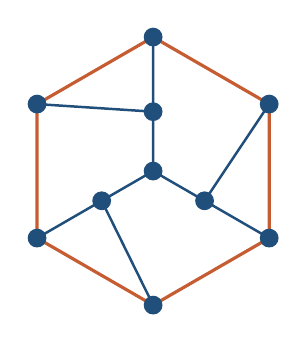
\begin{tikzpicture}[scale=0.92]
  \foreach \i in {0,...,5}
    \coordinate (l\i) at ({90-60*\i}:1.85);
  \coordinate (c) at (0,0);
  \coordinate (u0) at (90:0.82);
  \coordinate (u1) at (330:0.82);
  \coordinate (u2) at (210:0.82);
  \draw[added edge] (l0)--(l1)--(l2)--(l3)--(l4)--(l5)--cycle;
  \draw[edge] (c)--(u0) (c)--(u1) (c)--(u2);
  \draw[edge] (u0)--(l5) (u0)--(l0);
  \draw[edge] (u1)--(l1) (u1)--(l2);
  \draw[edge] (u2)--(l3) (u2)--(l4);
  \node[vertex] at (c) {};
  \foreach \p in {u0,u1,u2} \node[vertex] at (\p) {};
  \foreach \i in {0,...,5} \node[vertex] at (l\i) {};
\end{tikzpicture}
\end{center}
\classnote{Start with a plane tree having no degree-two vertex, then join its
leaves in cyclic order to form the highlighted rim.}
% lax end Lax68.HalinGraphs

\newpage

% lax begin Lax68.Wheels
\classheading{Wheels}
\begin{center}
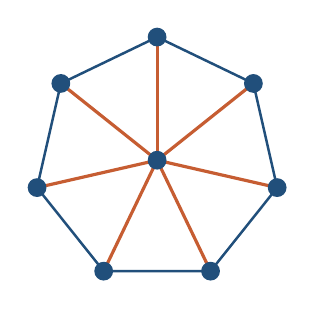
\begin{tikzpicture}[scale=0.92]
  \coordinate (h) at (0,0);
  \foreach \i in {0,...,6}
    \coordinate (v\i) at ({90-360*\i/7}:1.7);
  \draw[edge] (v0)--(v1)--(v2)--(v3)--(v4)--(v5)--(v6)--cycle;
  \foreach \i in {0,...,6} \draw[added edge] (h)--(v\i);
  \node[vertex] at (h) {};
  \foreach \i in {0,...,6} \node[vertex] at (v\i) {};
\end{tikzpicture}
\end{center}
\classnote{A rim cycle surrounds one universal hub, which is adjacent to
every rim vertex.}
% lax end Lax68.Wheels

% lax begin Lax68.SeriesParallel
\classheading{Series-parallel graphs}
\begin{center}
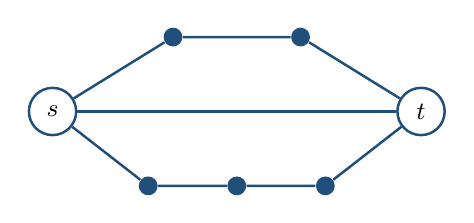
\begin{tikzpicture}[scale=0.9]
  \node[terminal] (s) at (-2.6,0) {$s$};
  \node[terminal] (t) at (2.6,0) {$t$};
  \node[vertex] (a) at (-0.9,1.05) {};
  \node[vertex] (b) at (0.9,1.05) {};
  \node[vertex] (c) at (-1.25,-1.05) {};
  \node[vertex] (d) at (0,-1.05) {};
  \node[vertex] (e) at (1.25,-1.05) {};
  \draw[edge] (s)--(t);
  \draw[edge] (s)--(a)--(b)--(t);
  \draw[edge] (s)--(c)--(d)--(e)--(t);
\end{tikzpicture}
\end{center}
\classnote{Series composition subdivides a terminal route; parallel
composition places terminal routes side by side between $s$ and $t$.}
% lax end Lax68.SeriesParallel

% lax begin Lax68.Trees
\classheading{Trees}
\begin{center}
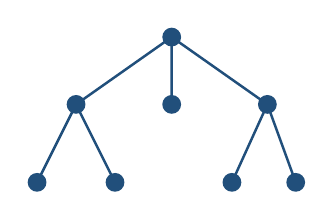
\begin{tikzpicture}[scale=0.9]
  \coordinate (r) at (0,1.6);
  \coordinate (a) at (-1.35,0.65);
  \coordinate (b) at (0,0.65);
  \coordinate (c) at (1.35,0.65);
  \coordinate (d) at (-1.9,-0.45);
  \coordinate (e) at (-0.8,-0.45);
  \coordinate (f) at (0.85,-0.45);
  \coordinate (g) at (1.75,-0.45);
  \draw[edge] (r)--(a) (r)--(b) (r)--(c);
  \draw[edge] (a)--(d) (a)--(e) (c)--(f) (c)--(g);
  \foreach \p in {r,a,b,c,d,e,f,g} \node[vertex] at (\p) {};
\end{tikzpicture}
\end{center}
\classnote{A tree is connected and contains no cycle; consequently there is
a unique path between every pair of vertices.}
% lax end Lax68.Trees

% lax begin Lax68.Paths
\classheading{Paths}
\begin{center}

\begin{tikzpicture}[scale=0.9]
  \foreach \x in {0,...,6} \node[vertex] (v\x) at (\x,0) {};
  \foreach \x [evaluate=\x as \y using int(\x+1)] in {0,...,5}
    \draw[edge] (v\x)--(v\y);
\end{tikzpicture}
\end{center}
\classnote{A path is a linear chain: two endpoints have degree one and every
internal vertex has degree two.}
% lax end Lax68.Paths

% lax begin Lax68.Triangulations
\classheading{Triangulations}
\begin{center}
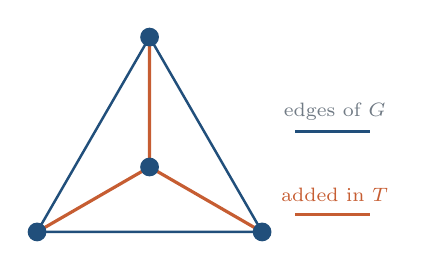
\begin{tikzpicture}[scale=1.0]
  \coordinate (a) at (90:1.65);
  \coordinate (b) at (210:1.65);
  \coordinate (c) at (330:1.65);
  \coordinate (d) at (0,0);
  \draw[edge] (a)--(b)--(c)--cycle;
  \draw[added edge] (d)--(a) (d)--(b) (d)--(c);
  \foreach \p in {a,b,c,d} \node[vertex] at (\p) {};
  \node[font=\scriptsize,graphgray] at (2.35,0.7) {edges of $G$};
  \draw[edge] (1.85,0.45)--(2.8,0.45);
  \node[font=\scriptsize,graphrust] at (2.35,-0.35) {added in $T$};
  \draw[added edge] (1.85,-0.6)--(2.8,-0.6);
\end{tikzpicture}
\end{center}
\classnote{A triangulation adds edges to a planar graph on the same vertex
set until no further edge can be added without losing planarity. In a plane
embedding, every face is then triangular.}
% lax end Lax68.Triangulations

\end{document}
